%! suppress = MissingImport
%! Author = maxwe
%! Date = 12.01.23

% Preamble
\documentclass{PyRollDocs}

% Packages
\usepackage{tabularray}
\UseTblrLibrary{booktabs}

\usepackage{symbols}

\newmintinline[py]{python}{}

% Document
\begin{document}

    \title{Documentation for the pyroll-ring-model-thermal Plugin}
    \author{Max Weiner}
    \date{\today}

    \maketitle


    \section{Model Description}\label{sec:model-description}

    \begin{figure}
        \centering
        \includegraphics[scale=0.8]{img/heat_flow}
        \caption{Heat Flows on a Disk Element Ring}
        \label{fig:heat_flow}
    \end{figure}

    \subsection{Ring Model}

    The following derivations are based on the ring model approach.
    For details on this approach read also the respective documentation\footnote{\url{https://github.com/pyroll-project/pyroll-ring-model}}.

    \subsection{Heat Flow Balance}

    As illustrated in \autoref{fig:heat_flow}, the heat flow balance of each ring on a disk element can be built as in \autoref{eq:heat_flow_balance}.

    \begin{equation}
        0 = \HeatFlow_{1\RingIndex} - \HeatFlow_{2\RingIndex} - \HeatFlow_{3\RingIndex} + \HeatFlow_{4\RingIndex} + \HeatSource{}_{\RingIndex}
        \label{eq:heat_flow_balance}
    \end{equation}

    The distinct heat contributions can be expressed as in the following.
    $\HeatFlow_{1\RingIndex}$ and $\HeatFlow_{2\RingIndex}$ are convective flows caused by workpiece material entry and exit in and from the disk element, where $\Density$ is the mass density, $\ThermalCapacity$ is the thermal capacity, $\VolumeFlow_\RingIndex$ the volume flow through the ring of the disk element, and $\Temperature_\RingIndex$ the absolute temperature of the respective ring.
    $\RingIndex$ is the index of the ring in the interval $[0, \RingIndexMax]$, where $\RingIndexMax = \RingCount - 1$ with the count of rings $\RingCount$.
    $\DiskIndex$, however, is the index of the disk, whose definition region is of no matter here.
    As all quantities except the temperatures are considered constant within one disk element, resp.\ ring, the index $\DiskIndex$ is neglected.
    But, all may vary from disk to disk.

    \begin{equation}
        \HeatFlow_{1\RingIndex} = \Density \ThermalCapacity \VolumeFlow_\RingIndex \Temperature_{\RingIndex}^{\DiskIndex}
        \label{eq:heat_flow_1}
    \end{equation}

    \begin{equation}
        \HeatFlow_{2\RingIndex} = \Density \ThermalCapacity \VolumeFlow_\RingIndex \Temperature_{\RingIndex}^{\DiskIndex+1}
        \label{eq:heat_flow_2}
    \end{equation}

    $\HeatFlow_{3\RingIndex}$ and $\HeatFlow_{4\RingIndex}$ are the conductive flows between the rings, with $\ThermalConductivity$ as the thermal capacity, $\Radius_\RingIndex$ as the radius coordinate of the rings center line, $\RadiusBoundary_\RingBoundaryIndex$ as the radius coordinates of the ring's boundaries and the disk width in rolling direction $\XWidth$.
    $\RingBoundaryIndex$ is the index of the ring boundary in the interval $[0, \RingBoundaryIndexMax]$, where $\RingBoundaryIndexMax = \RingIndexMax + 1$.

    \begin{equation}
        \HeatFlow_{3\RingIndex} = -\ThermalConductivity \frac{\Temperature_{\RingIndex+1}^{\DiskIndex}-\Temperature_{\RingIndex}^{\DiskIndex}}{\Radius_{\RingIndex+1} - \Radius_{\RingIndex}} \times 2 \pi \RadiusBoundary_{\RingIndex+1} \XWidth
        \label{eq:heat_flow_3}
    \end{equation}

    \begin{equation}
        \HeatFlow_{4\RingIndex} = -\ThermalConductivity \frac{\Temperature_{\RingIndex}^{\DiskIndex}-\Temperature_{\RingIndex-1}^{\DiskIndex}}{\Radius_{\RingIndex} - \Radius_{\RingIndex - 1}} \times 2 \pi \RadiusBoundary_{\RingIndex} \XWidth
        \label{eq:heat_flow_4}
    \end{equation}

    Heat generation by deformation is respected by the source term $\HeatSource$, with the efficiency of heat generation $\HeatSourceEfficiency$, the efficiency of deformation $\FormingEfficiency$, the flow stress $\FlowStress$ the deformed volume $\Volume$ and the equivalent strain rate $\StrainRate$.

    \begin{equation}
        \HeatSource{}_\RingIndex = \HeatSourceEfficiency \frac{\FlowStress}{\FormingEfficiency} \StrainRate \Volume_{\RingIndex}
        \label{eq:heat_source}
    \end{equation}

    The volume flow $\VolumeFlow$ through the ring is calculated from the cross section $\CrossSection_\RingIndex$ and the material flow velocity $\Velocity$.
    The velocity is approximated by the quotient $\frac{\XWidth}{\TimeWidth}$ with the time step $\TimeWidth$.
    This enables elimination of $\XWidth$ from the resulting equations, so the model becomes independent of the actual spacial axis in rolling direction.
    The step functions below are therefore formulated in terms of the time increment $\TimeWidth$.
    Especially in transport units the spacial axis may not be defined, but the time axis will.

    \begin{equation}
        \VolumeFlow_\RingIndex = \CrossSection_{\RingIndex} \Velocity = \CrossSection_{\RingIndex} \frac{\XWidth}{\TimeWidth}
        \label{eq:volume_flow}
    \end{equation}

    \noindent The cross-section of each ring is calculated as in \autoref{eq:cross_section}.
    Note, that $\RadiusBoundary_0 = 0$.

    \begin{equation}
        \CrossSection_{\RingIndex} = \pi \left( \RadiusBoundary_{\RingIndex+1}^2 -  \RadiusBoundary_{\RingIndex}^2 \right)
        \label{eq:cross_section}
    \end{equation}

    The outermost ring (surface ring) exchanges heat with the environment, so $\HeatFlow_{3,\RingIndexMax}$ is defined differently.
    The definition used here includes heat transfer according to a heat transfer coefficient concept and gray body radiation, with the heat transfer coefficient $\HeatTransferCoefficient$, the Stefan-Boltzmann radiation constant $\RadiationCoefficient$ and the relative radiation coefficient of the gray body $\RelativeRadiationCoefficient$.
    $\SurfaceTemperature$ is the absolute temperature of the surface.

    \begin{equation}
        \HeatFlow_{3\RingIndexMax} = \left[ -\HeatTransferCoefficient \left( \EnvironmentTemperature - \SurfaceTemperature \right) - \RadiationCoefficient\RelativeRadiationCoefficient\left( \EnvironmentTemperature^4 - \SurfaceTemperature^4 \right) \right]
        \times 2 \pi \RadiusBoundary_{\RingIndexMax+1} \XWidth
        \label{eq:heat_flow_3_surface}
    \end{equation}

    Since the surface is infinitesimally narrow, it has no heat capacity.
    Therefore, the heat flows on both sides must be equal.
    The $\SurfaceTemperature$ is approximated by equalizing the conductive flow from the outer ring and the heat transfer to the environment as in \autoref{eq:surface_temperature}.
    This is a scalar non-linear equation in $\SurfaceTemperature$ and can be solved f.e.\ by Newton's method.

    \begin{equation}
        \ThermalConductivity \frac{\SurfaceTemperature - \Temperature_\RingIndexMax^\DiskIndex}{\RadiusBoundary_{\RingIndexMax+1} - \Radius_{\RingIndexMax}} = \HeatTransferCoefficient \left( \EnvironmentTemperature - \SurfaceTemperature \right) + \RadiationCoefficient\RelativeRadiationCoefficient\left( \EnvironmentTemperature^4 - \SurfaceTemperature^4 \right)
        \label{eq:surface_temperature}
    \end{equation}

    \subsection{Temperature Increment Functions}

    Taking the equations shown above, the increment functions for the temperatures in each ring are formulated.
    $\TemperatureIncrement_\RingIndex = \Temperature_{\RingIndex}^{\DiskIndex+1} - \Temperature_{\RingIndex}^{\DiskIndex}$ is the respective temperature increment.
    The following equations are mostly equal for roll passes and transports, with the following differences:
    \begin{itemize}
        \item The heat transfer coefficients $\HeatTransferCoefficient$ take different values, as in transports convective heat flow is regarded and in roll passes solid body contact.
        \item In roll passes, radiation only occurs at the free surface at the sides of the profile and is negligible in comparison to the solid body contact, so $\RelativeRadiationCoefficient = 0$.
        \item In transport no deformation occurs, so $\StrainRate=0$ leading to a vanishing source term.
    \end{itemize}

    \noindent The core ring has no inner boundary, so $\HeatFlow_{40} = 0$.

    \begin{equation}
        \TemperatureIncrement_0 = \frac{\TimeWidth}{\Density\ThermalCapacity\CrossSection_0} \left[ \pi \ThermalConductivity \left( \Temperature_1^\DiskIndex - \Temperature_0^\DiskIndex \right) + \HeatSourceEfficiency \frac{\FlowStress}{\FormingEfficiency} \StrainRate \CrossSection_0 \right]
        \label{eq:increment_core}
    \end{equation}

    \noindent The intermediate rings take $\HeatFlow_{3\RingIndex}$ as in \autoref{eq:heat_flow_3}.

    \begin{equation}
        \TemperatureIncrement_\RingIndex = \frac{\TimeWidth}{\Density\ThermalCapacity\CrossSection_\RingIndex}
        \left[
        2 \pi \ThermalConductivity \left[
            \frac{\Temperature_{\RingIndex+1}^\DiskIndex - \Temperature_\RingIndex^\DiskIndex}{\Radius_{\RingIndex+1}-\Radius_{\RingIndex}}
            \RadiusBoundary_{\RingIndex+1}
            -\frac{\Temperature_{\RingIndex}^\DiskIndex - \Temperature_{\RingIndex-1}^\DiskIndex}{\Radius_{\RingIndex}-\Radius_{\RingIndex-1}}
            \RadiusBoundary_{\RingIndex}
            \right]
        + \HeatSourceEfficiency \frac{\FlowStress}{\FormingEfficiency} \StrainRate \CrossSection_{\RingIndex}
        \right]
        \label{eq:increment_layer}
    \end{equation}

    \noindent The surface ring takes $\HeatFlow_{3\RingIndexMax}$ as in \autoref{eq:heat_flow_3_surface} with respect to \autoref{eq:surface_temperature}.

    \begin{multline}
        \TemperatureIncrement_\RingIndexMax = \frac{\TimeWidth}{\Density\ThermalCapacity\CrossSection_\RingIndexMax}
        \Biggl[
        2 \pi \left[
            \left[ \HeatTransferCoefficient \left( \EnvironmentTemperature - \SurfaceTemperature \right) + \RadiationCoefficient\RelativeRadiationCoefficient\left( \EnvironmentTemperature^4 - \SurfaceTemperature^4 \right) \right]
            \RadiusBoundary_{\RingIndexMax+1}
            -\ThermalConductivity \frac{\Temperature_{\RingIndexMax}^\DiskIndex - \Temperature_{\RingIndexMax-1}^\DiskIndex}{\Radius_{\RingIndexMax}-\Radius_{\RingIndexMax-1}}
            \RadiusBoundary_{\RingIndexMax}
            \right] \\
        + \HeatSourceEfficiency \frac{\FlowStress}{\FormingEfficiency} \StrainRate \CrossSection_{\RingIndexMax}
        \Biggr]
        \label{eq:increment_surface}
    \end{multline}


    \section{Plugin Usage}\label{sec:plugin-usage}

    Load this plugin by

    \mint{python}{import pyroll.ring_model_thermal}

    To use this plugin, remember to define \py/Profile.density/, \py/Profile.thermal_capacity/, \py/Profile.thermal_conductivity/ on your input profile or as hook functions.

    If you are using disk elements, this plugin will calculate the temperature evolution stepwise on each disk element.
    Otherwise, the units will be treated as one step using the same equations as for a disk element.
    Therefore, the hook \py/Profile.ring_temperatures/ is implemented on the disk elements as well as on the respective unit's outgoing profiles, as listed below.

    If {pyroll.report} is installed, two types of plots are added to the report.
    For pass sequences, a plot displaying the evolution of surface, core and mean temperatures in dependence on the cumulative process time is generated similar to \autoref{fig:temperature_evolution_plot}.
    For disked units (currently roll passes and transports) a plot displaying the evolution of the temperature distribution within the unit is generated similar to \autoref{fig:temperature_profile_plot}.
    The latter shows the temperature curve of each profile in the unit (including the disk elements') indicated by color.
    The red curve indicates the in profile, the blue one the out profile.
    The disk elements' profiles are colored gradual between these two.
    This offers a pseudo-3D illustration of the temperature evolution.

    \begin{figure}
        \centering
        \begin{subfigure}[t]{0.48\linewidth}
            \centering
            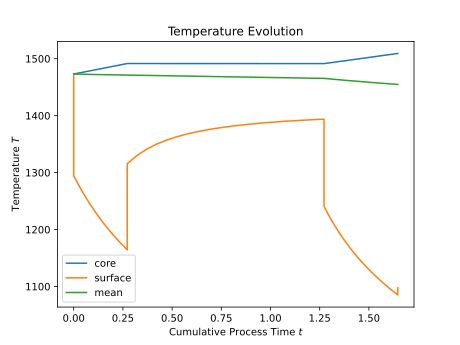
\includegraphics[width=\linewidth]{img/temperature_evolution_plot}
            \caption{Evolution of Key Temperatures Along a Pass Sequence}
            \label{fig:temperature_evolution_plot}
        \end{subfigure}
        \hfill
        \begin{subfigure}[t]{0.48\linewidth}
            \centering
            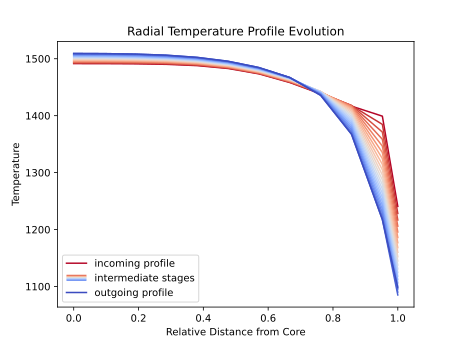
\includegraphics[width=\linewidth]{img/temperature_profile_plot}
            \caption{Evolution of the Temperature Distribution Within a Profile}
            \label{fig:temperature_profile_plot}
        \end{subfigure}
        \caption{Examples of Plots Added to the Report}
        \label{fig:report_plots}
    \end{figure}


    \section{Implementaion Details}

    The plugin provides several new hooks, as well as, additional hook functions for existing ones as listed below.
    Additionally to the listed ones, some technical hook functions are provided to copy data from incoming profiles and disk elements and other subunits.

    \py/Unit.OutProfile.temperature/ and \py/Unit.OutProfile.ring_temperatures/ are added to \py/root_hooks/.

    \subsection{Profiles}

    \subsubsection{Additional Hooks}

    \begin{description}
        \item[\py/Profile.ring_temperatures/] a numpy array of the rings' local temperatures according to the ring model standard
    \end{description}

    \subsubsection{Provided Implementations}

    \begin{description}
        \item[\py/Profile.ring_temperatures/] creates the \py/Profile.ring_temperatures/ array from a single \py/Profile.temperature/ value as a homogeneous state.
        Meant mainly for creation of an initial state, if only a single temperature is given on the input profile.
        \item[\py/Profile.temperature/] calculates the nominal temperature of the profile as arithmetic mean of the ring temperatures
        \item[\py/Profile.surface_temperature/] returns the outer ring's temperature as approximation for the surface temperature, if no further information is given.
        This implementation is overridden by the implementations of the respective unit profiles.
        \item[\py/core_temperature/] returns the core ring's temperature as core temperature
    \end{description}

    \subsection{Roll Passes}

    \subsubsection{Additional Hooks}

    \begin{description}
        \item[\py/RollPass.heat_transfer_coefficient/] represents the heat transfer coefficient $\HeatTransferCoefficient$ for the contact of workpiece and rolls, implemented with default value \qty{6000}{\watt\per\squared\meter\per\kelvin}
        \item[\py/RollPass.deformation_heat_efficiency/] represents the efficiency of heat generation by deformation $\HeatSourceEfficiency$, implemented with default value \num{0.95}
    \end{description}

    \subsubsection{Provided Implementations}

    \begin{description}
        \item[\py/RollPass.OutProfile.ring_temperatures/]
        \item[\py/RollPass.DiskElement.OutProfile.ring_temperatures/] calculates the temperature evolution according to the equations \autoref{eq:increment_core}, \autoref{eq:increment_layer} and \autoref{eq:increment_surface} as described above
        \item[\py/RollPass.Profile.surface_temperature/]
        \item[\py/RollPass.DiskElement.Profile.surface_temperature/] calculates the surface temperature by solving \autoref{eq:surface_temperature} as described above
    \end{description}

    \subsection{Transports}

    \subsubsection{Additional Hooks}

    \begin{description}
        \item[\py/Transport.heat_transfer_coefficient/] represents the heat transfer coefficient $\HeatTransferCoefficient$ for convection transfer to the atmosphere, implemented with default value \qty{15}{\watt\per\squared\meter\per\kelvin}
        \item[\py/Transport.relative_radiation_coefficient/] the relative radiation coefficient $\RelativeRadiationCoefficient$, implemented with default value \num{0.8}
    \end{description}

    \subsubsection{Provided Implementations}

    \begin{description}
        \item[\py/Transport.OutProfile.ring_temperatures/]
        \item[\py/Transport.DiskElement.OutProfile.ring_temperatures/] calculates the temperature evolution according to the equations \autoref{eq:increment_core}, \autoref{eq:increment_layer} and \autoref{eq:increment_surface} as described above
        \item[\py/Transport.Profile.surface_temperature/]
        \item[\py/Transport.DiskElement.Profile.surface_temperature/] calculates the surface temperature by solving \autoref{eq:surface_temperature} as described above
    \end{description}

%    \addsec{Symbols}

\begin{longtblr}[
    label= none,
    entry = none
]{ll}
    \toprule
    Symbol & Description \\
    \midrule
    
    ${{s["code"]}}$ & {{s["descr"]}}\\
    
    \bottomrule
\end{longtblr}

    \printbibliography


\end{document}